\documentclass[10pt,a4paper]{article}

\usepackage[spanish]{babel}
\usepackage[utf8]{inputenc}
\usepackage{geometry}
\usepackage{url}
\usepackage{amsmath}
\usepackage{graphicx}
\usepackage{float}
\usepackage{listings}
\usepackage{color}
\usepackage{multicol}
\definecolor{grey}{rgb}{0.8,0.8,0.8}
\usepackage{listings}
\usepackage{color,soul}
\usepackage{caption}
\usepackage{subcaption}
%\usepackage{bibtex}
\usepackage{multirow}
\usepackage{float}


% Macros
% #1 : Path of image. eg : window/aWindow.png
% #2 : Caption of image. eg : a caption
% #3 : Width of image in centimeters. eg : 15
% #4 : Height of image in centimeters. eg : 20
% 
% example : \presentgrafic{window/aWindow.png}{caption}{15}{20}
\newcommand{\presentgrafic}[4]{
\begin{figure}[H]
\centering
\includegraphics[width=#3cm, height=#4cm]{#1}
\caption{#2}
\label{fig:my_label}
\end{figure}
}
\lstset{
  frame=top,frame=bottom,
  basicstyle=\footnotesize\normalfont\ttfamily,%\sffamily,    % the size of the fonts that are used for the code
  stepnumber=1,                           % the step between two line-numbers. If it is 1 each line will be numbered
  numbersep=10pt,                         % how far the line-numbers are from the code
  tabsize=2,                              % tab size in blank spaces
  extendedchars=true,                     %
  breaklines=true,                        % sets automatic line breaking
  captionpos=t,                           % sets the caption-position to top
  mathescape=true,
  stringstyle=\color{white}\ttfamily, % Farbe der String
  showspaces=false,           % Leerzeichen anzeigen ?
  showtabs=false,             % Tabs anzeigen ?
  xleftmargin=17pt,
  framexleftmargin=17pt,
  framexrightmargin=17pt,
  framexbottommargin=5pt,
  framextopmargin=5pt,
  showstringspaces=false      % Leerzeichen in Strings anzeigen ?
 }

\begin{document}

\begin{titlepage}

\newcommand{\HRule}{\rule{\linewidth}{0.5mm}} % Defines a new command for the horizontal lines, change thickness here

\center % Center everything on the page

\textsc{\LARGE Facultad de Ingeniería - UBA}\\[1.5cm]
\textsc{\Large Organización de Datos 75.06}\\[0.5cm]
\textsc{\large Trabajo Práctico: Informe Final}\\[0.5cm]

\HRule \\[0.4cm]
{ \huge \bfseries Fine Food Reviews}\\[0.4cm]
\HRule \\[1.5cm]

\begin{minipage}{0.5\textwidth}
\begin{flushleft} \large
\emph{Integrantes:}\\
Agustina \textsc{Barbetta} \textit{96528}\\
Santiago \textsc{Lazzari} \textit{96735}\\
Luciano \textsc{Mintrone} \textit{95463}\\
Manuel \textsc{Porto} \textit{96587}\\
\end{flushleft}
\end{minipage}
~
\begin{minipage}{0.4\textwidth}
\begin{flushright} \large
\emph{E-mails:}\\
\texttt{agustina.barbetta@gmail.com}\\
\texttt{santilazzari1994@gmail.com}\\
\texttt{lucianomintrone@gmail.com}\\
\texttt{manu.porto94@gmail.com}\\
\end{flushright}
\end{minipage}\\[2cm]

{\Large \texttt{Grupo 18}}\\[2cm]

\selectlanguage{spanish}
{\large \today}\\[3cm]

\begin{abstract}
En el presente trabajo se implementa un predictor de puntaje para un set de datos con reseñas de productos estudiado, anteriormente, en la instancia de diseño.
\end{abstract}

\vfill

\end{titlepage}

\tableofcontents

\pagebreak

\section{Modelo propuesto anteriormente}

\subsection{Pre-procesamiento}
Para la solución a implementar se decidió realizar una eliminación del HTML, caracteres especiales, numéricos y pasaje a lower case sobre los sets \textit{training} y \textit{test}, obviando la eliminación de \textit{stopwords}, ya que desempeñan una función importante a la hora de entender los sentimientos de los usuarios.

Se propone realizar un manejo de las negaciones. Al utilizar cada palabra como un \textit{feature}, la palabra ``good'' en la frase ``not good'' contribuirá a un sentimiento positivo en lugar de a uno negativo, debido que la presencia de ``not'' no se tiene en cuenta. Para resolver este problema se escribirá un \textit{script} que transforme una palabra seguida de un ``not'' o ``n't'' en ``not\_'' + palabra. Las palabras a negar se detectan con una variable de estado, cuando esta es verdadera, a todas las palabras leídas se les antepondrá la negación. La variable vuelve a su valor inicial cuando se encuentra un signo de puntuación u otra negación. %recordar cambiar el preprocess para que deje ' y .

\subsection{Procesamiento}
%\hl{Cambie ProductId por Id, pero no se si corresponde cambiarlo aca (porque esto es lo que ya propusimos en el diseno, o directamente explicar el cambio en las secciones posteriores}

Previo al entrenamiento del modelo elegido, se deberá preparar el set de acuerdo a los requisitos del algoritmo. Además se determinará qué campos serán incluidos para realizar el entrenamiento, en base a lo explicado en apartados anteriores.

El procesamiento propuesto consiste en construir una matriz compuesta por los Id's de las reseñas, su puntaje y todas las palabras halladas en los campos ``Summary'' y ``Text'' de  todas las reviews. Cada fila de esta matriz corresponde a un review individual. Cada una de las palabras corresponderá a un atributo y tendrán un valor entre 0 y N dependiendo de la cantidad de veces que dicha palabra aparezca en la review. A continuación se presenta un ejemplo de la matriz:

\begin{table}[H]
    \centering
    \begin{tabular}{|ccccc|}
    \hline
     Id& Prediction & good & not\_good & taste \\ \hline \hline
     1 & 4 & 3 & 0 & 1 \\
     2 & 1 & 0 & 2 & 2 \\
     3 & 2 & 1 & 3 & 0\\
     4 & 2 & 0 & 1 & 0\\ \hline
    \end{tabular}
    \caption{}
\end{table}

Dado que la gran cantidad de palabras existentes tiene como consecuencia que las matrices tengan una dimensión demasiado grande, se filtrarán las palabras en base a su ocurrencia. Sabiendo que la cardinalidad de las palabras por predicción se distribuye como una ley de potencias, se podrá encontrar algún porcentaje empírico de palabras, las más relevantes, que se utilizarán para entrenar. Y siendo ésta distribución una ley de potencias, dicha relación es invariante a la escala, es decir, que para todas las predicciones (independientemente de la cantidad de reviews que tengan) se podrá usar la mismo proporcionalidad.

Otra forma de reducir éste número es aplicarle the hashing trick a las palabras y así poder reducir las dimensiones de la matriz. Se probará si hace falta aplicarle the hashing trick, y si hiciera falta, cuán costoso és. 

\subsection{Predicción}
El modelo que se utilizará para predecir el puntaje de los reviews será SVM, como ya se explicó, SVM es un algoritmo especialmente útil para clasificación de textos. Este modelo puede ser utilizado para problemas no lineales, como es el caso del presente trabajo \cite{svm_crammer} y se cuenta con evidencia empírica de que obtiene mejores resultados que otros algoritmos para problemas de clasificación no lineales. \cite{svm_thorsten}

Según lo investigado, SVM no funciona bien para sets de datos desbalanceados\cite{quora}, lo cual es nuestro caso (como fue detallado en el análisis del set de datos). Para solucionar este problema se pueden usar dos alternativas; Una solución posible es balancear el set de datos, recortándolo aleatoriamente o aprovechando a sacar las entradas repetidas. Por otro lado, si esto último no funciona, optaremos por cambiar el predictor por otro, como un perceptrón multicapa.

\section{Flujo y procesamiento de la información}
El dataset es procesado de la siguiente manera:

\begin{enumerate}
    \item Se preprocesan los reviews del set con el script de PySpark, \texttt{parallel\_preprocess.ipynb}. En el se realizan los siguiente cambios, que luego son guardados en un nuevo archivo. 
        \begin{itemize}
            \item Eliminación de HTML
            \item Eliminación de caracteres especiales
            \item Eliminación de caracteres numéricos
            \item Pasaje a lower case
            \item Eliminación de stopwords
            \item Negador
        \end{itemize}
    
    %\item Realizar un segundo preprocess en donde se junta el texto de Summary con la review en si y se expanden las palabras negadas (\textit{ej don\'t}) en la palabra y su negador por separado. \hl{Updatear esto cuando se mergeen los preprocess}.
    \item Una vez pre-procesado se vectoriza el texto de cada review y se reducen las dimensiones de los vectores resultantes mediante Hashing Trick con el script \texttt{word2matrix.py}.
    \item Se utiliza la totalidad del \textit{training} set como entrenamiento para el clasificador.
    \item Realizado el entrenamiento, se utiliza el \textit{test} set para generar las predicciones.
\end{enumerate}

%El set para predecir se trata de la misma forma, pero una vez que tiene el formato adecuado para la red neuronal, se lo utiliza con esta ultima para generar las predicciones.

\section{Pre-procesamiento}
El script parte de los sets de datos descargados de Kaggle y consiste en pasar los campos Summary y Text de una review por una función que recibe una cadena y ejecuta una serie de funciones sobre ella.

En primer lugar, tres expresiones regulares que filtran el marcado HTML, los caracteres especiales (Excepto los . y ', que se necesitarán para el manejo de negaciones) y los caracteres numéricos.
Luego, se pasa toda la cadena a lower case y se la recorre para eliminar las palabras que se encuentran en nuestro \texttt{stopwords.csv} en el cual hemos puesto las palabras que no contienen un significado importante para el idioma inglés, excluyendo palabras como ``good'',``like'', ``not'' ya que estas pueden aportar la predicción del sentimiento del usuario.  
Por último, se realiza la negación de la cadena, que transforma cada palabra seguida de un ``not'' o ``n't'' en ``not\_'' + palabra. Las palabras a negar se detectan con una variable de estado; cuando esta es verdadera, a todas las palabras leídas se les antepone la negación. La variable vuelve a su valor inicial cuando se encuentra un signo de puntuación u otra negación.
Opcionalmente, se añaden los pasos de \textit{stemming}, que lleva cada palabra de la cadena a su raíz, y \textit{n-gram}, que realiza secuencias de n palabras con la review. 

\section{Procesamiento}
Para este paso, se parte de los sets de datos pre-procesados y se vectoriza cada review de ambos sets por medio de \textbf{Hashing Trick}.

Luego del estudio realizado para la entrega de diseño (vimos, por ejemplo, que los usuarios suelen escribir reviews de longitudes similares independientemente del puntaje que le asignen a un producto (Figura \ref{fig:rev_len}) y que los \textit{HelpfulnessNumerator} y \textit{HelpfulnessDenominator} no suelen marcar diferencias ya que son muy pocos los votos totales por review (Figura \ref{fig:hdenom})), decidimos procesar sólo los campos \textit{Summary} y \textit{Text} de los sets de datos.

Inicialmente se decidió convertir los textos del set a vectores con una cota de error del 1\% que, según el teorema de Johnson-Linderstrauss, son de 127 dimensiones. Más adelante fuimos probando con mayores dimensiones reduciendo, consecuentemente, la cota del error.

La salida de este script es un \texttt{.csv} con \texttt{Id,Prediction,vector} en el caso del \textit{training} set y \texttt{Id,vector} en el caso del \textit{test} set.

\begin{figure}
\centering
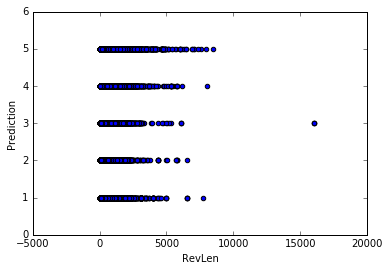
\includegraphics[scale=0.7]{revlen}
\caption{Longitud de reviews por puntuación}
\label{fig:rev_len}
\end{figure}

\begin{figure}
\centering
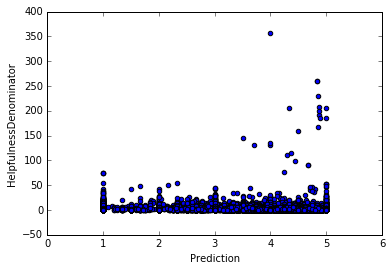
\includegraphics[scale=0.7]{hdenom}
\caption{\textit{HelpfulnessDenominator} por puntuación}
\label{fig:hdenom}
\end{figure}
\section{Predictores utilizados}

\subsection{Support Vector Machines}
Si bien en la entrega de diseño propusimos la utilización de este algoritmo, al momento de implementarlo encontramos que las implementaciones presentes no eran óptimas para las condiciones de nuestro problema. En una de las librerías de análisis de datos de Python advertían que su implementación no escalaba bien para un numero de muestras mayor a 10000 ya que su implementación del algoritmo es de orden cuadrático. \cite{sklearn_svc}

Teniendo en cuenta lo anterior consideramos que utilizar dicha librería no seria adecuado para el presente problema. Si bien podríamos haber implementado nuestra propia versión, consideramos que dado el tiempo disponible y los conocimientos que teníamos sobre el tema, la tarea no era factible por lo que decidimos no utilizar este algoritmo.

\subsection{Dynamic Vector Prediction}

Inspirados en la charla de las JAIIO y de la manera en que Facebook hacia sentiment analisis, propusimos un algoritmo similar que lo llamamos Dynamic vector prediction.

El algoritmo consiste en armar una tabla de la forma palabra:cardinalidad de la palabra por cada predicción. Por ejemplo, en el caso de la predicción 1.

\begin{lstlisting}[firstnumber=1]
    {
    "tast":22508,
    "br":22305,
    "like":21614,
    "product":21051,
    "one":15308,
    "food":14724
    .
    .
    .
    }
\end{lstlisting}

Esto se genera recorriendo todos los reviews y de una misma predicción y sumando 1 por cada palabra. Ésta tabla de frecuencias seria el equivalente al aprendizaje.

Para poder predecir un review por ejemplo ``The food was awful'' 

Se hace un split lo cual queda [``The'', ``food'' ,  ``was'',  ``awful'' ]. Teniendo esto que llamaremos, la referencia, se genera un vector, llamado vector dinámico con la cardinalidad de cada palabra. Es decir, si alguna palabra se repitiera, no estaría duplicada en las referencias pero si aumentaría la cardinalidad en el vector dinámico. En este caso el vector dinámico quedaría de la siguiente forma. [1, 1, 1, 1]. 

Teniendo las tablas de frecuencias de las 5 predicciones, se hace lo mismo con las palabras de referencia. Por ejemplo, si ``The'' tiene cardinalidad 10000, ``food'' 1500,``was'' 10000 y ``awful''500, en la predicción 1 entonces el vector dinámico es [10000, 1500, 1000, 500]. Esto se repite con todas las predicciones.

A esta altura se generaron 6 vectores dinámicos, el de la review + las 5 predicciones. Para poder comprar todos los reviews de la misma forma, sabiendo que el set de datos está desbalanceado, se procede a normalizar los 6 vectores.

Finalmente se calcula la distancia coseno entre la review contra todas las predicciones y se queda con la menor. Esto define a cuál se parece más y esa es la predicción.


Los resultados de éste algoritmo se probaron con tres distancias distintas y se hizo un post en Kaggle con la mejor de ellas. Basándonos en cuánto se ajustaba al train set.

Con la distancia del coseno los resultados fueron 377 predicciones correctas con respecto a mil. Con la Euclideana fueron 345. Mientras que con Jaccard 77.

Se obtuvo una puntuación de \texttt{5.06451} en Kaggle, por lo que concluimos en que el algoritmo no es bueno para este tipo de problema.


\subsection{Perceptrón}
Como sabemos perceptrón es un clasificador binario lineal por lo tanto tuvimos que adaptarlo a nuestro problema que tiene mas de dos clases. Para ello propusimos perceptrones en cascada, en donde el primero de ellos divide el las reseñas es buenas (3,4 y 5 estrellas) y malas (1 y 2 estrellas). Luego aplicamos un nuevo perceptrón dentro de las reseñas malas, obteniendo una lista de reseñas de 1 estrella y otra lista de 2 estrellas. Lo mismo se realizo para las buenas reseñas. 
Mediante Cross Validation fuimos probando los resultados y cambiando los hiperparámetros dependiendo de estos. Los hiperparámetros a modificar son la función de activación, el numero de dimensiones de los datos, la cantidad de iteraciones para entrenar el vector de pesos. 
Usando la función de activación sigmoid, 127 dimensiones y 10 iteraciones obtuvimos un resultado de 50\% de resultados correctos con Cross Validation y en Kaggle de \texttt{5.13634}


\subsection{Red Neuronal}
Inspiradas en las redes neuronales biológicas, una red multicapa utiliza el concepto de los perceptrones donde cada perceptrón es una neurona de una red que conecta varias de estas unidades.

Dado que la red puede ser entrenada con hiperparámetros y datos procesados de distintas formas, se realizaron pruebas con algunas de las combinaciones posibles.
\begin{enumerate}
    \item Random search de mejores hiperparámetros.
    \item Separando el campo \textit{Summary} de \textit{Text}. se subieron entradas aplicando pesos mayores a \textit{Summary} y con pesos idénticos para ambos.
    \item Recortando los \textit{reviews} de 5 estrellas del \textit{training} set a $1/3$.
    \item Reduciendo cantidad de iteraciones para evitar \textit{overfitting}.
    \item Aumentando la cantidad de dimensiones del vector de The Hashing Trick.
    \item Realizando bigramas antes de vectorizar las reviews.
\end{enumerate}

\subsubsection{Random search de hiperparámetros óptimos}
Primero se entrenaron y validaron, con Cross Validation, redes con distintos hiperparámetros y el mismo set de datos. Los parámetros fueron los siguientes.

\begin{enumerate}
    \item activations = ['identity', 'logistic', 'tanh']
    \item solvers = ['lbfgs', 'sgd', 'adam']
    \item learning\_rates = ['constant', 'invscaling', 'adaptive']
    \item layers : De 1 a 10 layers cada una con 10 a 100 neuronas
    \item alpha : Un numero del 0 al 1
    \item momentum : Un numero próximo a 0.9
    \item beta\_1 : Un número próximo al 0.9
    \item beta\_2 : Un número muy próximo al 0.9
\end{enumerate}


Luego se tomaron las mejores dos redes y se utilizaron las mismas para realizar dos entregas a Kaggle.
Los puntajes fueron \texttt{4.90687} para 

\begin{lstlisting}
Net ID 25 Correct prediction 33774 total predictions 45468 ratio 
       0.742808128794

MLPClassifier(activation='relu', alpha=6.4603656567e-05, batch_size='auto',
       beta_1=0.762066045724, beta_2=0.9977827051, early_stopping=False,
       epsilon=1e-08, hidden_layer_sizes=(82, 63, 62, 82, 84, 14, 17, 94),
       learning_rate='adaptive', learning_rate_init=0.001, max_iter=200,
       momentum=0.802854594112, nesterovs_momentum=True, power_t=0.5,
       random_state=1, shuffle=True, solver='adam', tol=0.0001,
       validation_fraction=0.1, verbose=True, warm_start=False)
\end{lstlisting}

y \texttt{4.77462} para

\begin{lstlisting}
Net ID 17 Correct prediction 32056 total predictions 45559 ratio        
      0.703615092517

MLPClassifier(activation='relu', alpha=1.81461856718e-05, batch_size='auto',
      beta_1=0.647482014388, beta_2=0.9977827051, early_stopping=False,
      epsilon=1e-08, hidden_layer_sizes=(35, 73, 90, 24, 47, 66, 18, 38),
      learning_rate='constant', learning_rate_init=0.001, max_iter=200,
      momentum=0.648414985591, nesterovs_momentum=True, power_t=0.5,
      random_state=1, shuffle=True, solver='adam', tol=0.0001,
      validation_fraction=0.1, verbose=True, warm_start=False)
\end{lstlisting}

Para visualizar los parametros de las redes recien mencionadas y el resto de las utilizadas en el \textit{Random Search} se debe acceder al archivo de analisis de los mismos, presente en el repositorio del trabajo.\cite{random_search}
\subsubsection{Pesos idénticos para Summary y Text}
Con 40 iteraciones, vectorizamos las reviews utilizando el Hashing Trick explicado anteriormente, entrenamos la red y la utilizamos para predecir. Se obtuvo una puntuación de \texttt{2.04606} en Kaggle.

\subsubsection{Peso doble para Summary}
Manteniendo constante el número de iteraciones (40) y teniendo en cuenta que el campo \textit{Summary} es el título de la review, se nos ocurrió ponderarlo con un peso mayor frente al campo \textit{Text} ya que, el primero, es un resumen del segundo.

Para ello, modificamos nuestro vectorizador de textos para que incremente en dos unidades la dimensión indicada por la función de hash cuando se vectorizan palabras del campo \textit{Summary}. Mientras que dejamos que incremente una unidad para las dimensiones hasheadas por palabras en el campo \textit{Text}.

Se obtuvo una puntuación de \texttt{2.21231} en Kaggle. La cual es peor que en los intentos anteriores, por lo que descartamos esta idea y continuamos ponderando los features \textit{Summary} y \textit{Text} de la misma forma.

\subsubsection{Recorte de 2/3 de las reviews puntuadas con 5}
Frente al desbalance del set de entrenamiento estudiado para la entrega de diseño (En el cual vimos que un 75\% de las reviews tienen \textit{Prediction} 5), decidimos probar entrenando la red excluyendo 2/3 de estas reviews.
Las mismas fueron vectorizadas mediante el Hashing Trick usual con un peso equitativo para los campos \textit{Summary} y \textit{Text}, y estos vectores utilizados para entrenar la red neuronal con 40 iteraciones.
Se obtuvo una puntuación de \texttt{2.08896} en Kaggle. La cual es peor que en el intento anterior (con el set completo), por lo que se descartó esta idea.

\subsubsection{Reducción de iteraciones realizadas durante entrenamiento de la red}
Consideramos que las redes estaban fallando en generalizar correctamente, debido a que estaban realizando una gran cantidad de iteraciones al momento de entrenarse. Por lo tanto, decidimos reducir la cantidad de las mismas para resolver este problema (De 40 a 25). 
Se obtuvo una puntuación de \texttt{2.04423} en Kaggle. La puntuación de la entrega fue superior, por lo que se consiguió una mejora en la capacidad de predicción de la red. Al ver una mejora, continuamos entrenando con pocas iteraciones.

\subsubsection{Texto de reseñas agrupados en bigramas}
Una variante utilizada fue agrupar el texto de las reviews en bigramas durante el pre-procesamiento. Se vectorizaron las reviews con 127 dimensiones y se iteró 25 veces sin embargo esto no produjo mejores resultados a los ya obtenidos. La puntuación en Kaggle fue de \texttt{2.32407}.

Se intentó pre-procesar con n-gramas mayores sin éxito por problemas de \textit{timeout} en PySpark.

\subsubsection{Utilización de tabla de hash de mayor dimensión}
Para reducir el numero de colisiones y por consiguiente el error asociado al vectorizar las reseñas decidimos incrementar el tamaño de la tabla de hash utilizada de 127 a 1009. Proseguimos a entrenar la red con 25 pasadas. Este cambio logró una mejora significativa en la precisión de la red ya que se logró una puntuación de \texttt{1.02591}. Continuamos aumentando la cantidad de dimensiones, esta vez de 1009 a 1511. Entrenamos la red con 25 pasadas y obtuvimos un resultado de \texttt{0.90247} en Kaggle.

Continuamos aumentando la cantidad de dimensiones a 2003, pero la computadora utilizada no disponía de la cantidad de memoria suficiente para realizar la tarea, por lo que no fue posible entrenar la red con esta cantidad de dimensiones.

Luego, realizamos un intento modificando la cantidad de iteraciones de 25 a 40 con 1511 dimensiones, cuyo resultado fue de \texttt{0.91549}.

Finalmente, realizamos un último intento con 25 iteraciones y 1709 dimensiones, pero el resultado fue el mismo que en el caso de las 2003 dimensiones. 

\subsection{Naïve Bayes}
Como describimos en el diseño Naïve Bayes es una extensión de Bayes para n características, las cuales se asumen independientes. Aplicamos su formula
\begin{equation*}
    P(y|x_1,..,x_n) = \frac {P(y)\prod_{i = 1}^{n} {P(x_i|y)}} {P(x_1,..,x_n)}
\end{equation*}

En donde 'y' seria la puntuación y 'x' cada \textit{feature} que en nuestro caso corresponde a cada palabra. Entonces vamos a calcular a 

\begin{enumerate}
    \item P(y) como la $\frac {review-de-clase-x}{total-de-reviews}$
    \item $P(x|y)$ como la frecuencia de la palabra x en la clase y $ p_{palabra} = \frac{apariciones}{total} $ 
    \item $P(x_1,..,x_n)$ como la probabilidad de que en un review aparezcan esas palabras.
\end{enumerate}

Luego vemos para cada clase cual tiene mas probabilidad de ser elegida. El resultado en Cross Validation no es muy bueno siendo al rededor del 28\% 
Una desventaja de este algoritmo es que no puede ser entrenado, una forma de mejorarlo es consiguiendo mas datos, que por otro lado lo hace mas lento.

Mediante algoritmo se obtuvo una puntuación de \texttt{2.68657} en Kaggle. Dicha puntuación se condice con el resultado de Cross Validation, que no era bueno. 

\subsection{Decision Trees}
Otro de los algoritmos utilizados fue el de Arboles de Decisión. Si bien este algoritmo no fue propuesto en la entrega de diseño, al ser un algoritmo sencillo de utilizar y con un orden de ejecución logarítmico \cite{sklearn_dtree} consideramos interesante probar este algoritmo y compararlo con nuestras otras soluciones.

Se realizaron dos pruebas con este algoritmo, en ambas se entreno al árbol con los parámetros por defecto del mismo pero se modificaron las dimensiones utilizadas durante la vectorización de los sets de datos. En la primer prueba se utilizaron 129 dimensiones y se obtuvo un resultado de \texttt{1.77059}, mientras que en la segunda se aumento las dimensiones del mismo a 1009 y logramos un resultado de \texttt{1.32765}. Al igual que en la red neuronal, el aumento de dimensiones durante \textit{Hashing Trick} impacta positivamente en la precisión del modelo ya que se reduce el error por colisiones de palabras distintas.

Es importante notar que este modelo es susceptible a sets de datos desbalanceados \cite{sklearn_dtree}, como el utilizado en el presente trabajo, por lo que los resultados podrían haber sido mejores en el caso de haber entrenado al árbol con un set balanceado. Sin embargo, por limitaciones de tiempo no fue posible realizar esta prueba por lo que no podemos afirmar cuan significativa hubiese sido la mejora de la predicción.

\subsection{Tabla de submits realizados en Kaggle}
\begin{table}[H]
\centering
\label{tabla}
\begin{tabular}{|l|l|ll|}
\hline
\multicolumn{3}{|l}{\textbf{Predictor}}                                                                                            & \multicolumn{1}{l|}{\textbf{Puntaje}} \\ \hline
\multicolumn{3}{|l}{Vowpal Wabbit}                                                                                                 & 0.41703                               \\ \hline
\multicolumn{3}{|l}{Dynamic Vector Prediction}                                                                                     & 5.06451                               \\ \hline
\multicolumn{3}{|l}{Naive Bayes}                                                                                                   & 	2.68657                              \\ \hline
\multicolumn{3}{|l}{Perceptrón}                                                                                                    & 5.13634                               \\ \hline
\multirow{2}{*}{Decision Trees}                                                                                                & \multicolumn{2}{l}{Hashing Trick de 127 dimensiones} 
                                                                        & 1.77059                   \\ \cline{2-4}
                                        & \multicolumn{2}{l}{Hashing Trick de 1009 dimensiones} 
                                                                        & 1.32765 
                                                        \\ \hline
\multirow{9}{*}{Red Neuronal} & \multicolumn{2}{l}{Random Search de hiperparámetros}                                                                            & 4.77462                                                          \\ \cline{2-4} 
                              & \multicolumn{2}{l}{Pesos idénticos para Summary y Text}                                            & 2.04606                               \\ \cline{2-4} 
                              & \multicolumn{2}{l}{Peso doble para Summary}                                                        & 2.21231                               \\ \cline{2-4} 
                              & \multicolumn{2}{l}{Recorte de 2/3 de las reviews puntuadas con 5}                                  & 2.08896                               \\ \cline{2-4} 
                              & \multicolumn{2}{l}{Reducción de iteraciones}                                                       & 2.04423                               \\ \cline{2-4} 
                              & \multicolumn{2}{l}{Preprocesamiento con bigramas}                                                  & 2.32407                               \\ \cline{2-4} 
                              & \multirow{3}{*}{Aumento de las dimensiones en Hashing Trick} & 1009 dim. 25 iter. & 1.02591                               \\ \cline{3-4}
                              &                                                                  & 1511 dim. 25 iter. & 0.90247                               \\ \cline{3-4} 
                              &                                                                  & 1511 dim. 40 iter. & 0.91549                               \\ \hline
\end{tabular}
\caption{Tabla de submits realizados en Kaggle}
\end{table}

\section{Algoritmo final utilizado}
% Indiquen el algoritmo final usado. Cambios realizados con respecto a la entrega de diseño.
Como explicamos a lo largo del informe, no nos limitamos a utilizar un solo algoritmo sino que probamos prediciendo las reviews con varios. Sin embargo, al encontrar un predictor con un mejor resultado inicial, como lo fue Redes Neuronales, nos dedicamos a ahondar en el mismo modificando no sólo sus hiperparámetros sino también el previo pre-procesamiento y vectorización de los datos. 

Como se puede ver en la tabla de puntuaciones, nuestros mejores resultados fueron obtenidos con pre-procesamiento sin \textit{stemming} ni n-gramas, muchas dimensiones al realizar Hashing Trick (Entre 1000 y 1500 que fue el máximo que pudimos probar con éxito) y pocas iteraciones al entrenar la red (Alrededor de 25, para que la red no se ajuste a predecir sólo el \textit{training} set). 

Cabe destacar que luego de explotar los recursos de la red también obtuvimos muy buenos resultados, desde el principio, con Decision Trees para el cual también mejoró el puntaje significativamente al aumentar la cantidad de dimensiones de la vectorización de reviews.

% intenso guitarreo en esta seccion, cambien lo que quieran c:

\section{Comentario final}
% Breve comentario final sobre el TP: experiencia obtenida, cosas que aprendieron, si les pareció interesante, resultados, etc

En términos generales, notamos que al mantener el modelo lo más simple posible se obtuvieron los mejores resultados, es decir sin aplicar transformaciones como \textit{stemming}, \textit{shingles}, etcétera a los datos. 

Por otro lado, pudimos observar que las pruebas que daban bien con el \textit{training} set no necesariamente lo hacían con el set de prueba. Esto ocurría porque el algoritmo no  generalizaba correctamente a causa del \textit{over-fitting}. La solución propuesta fue iterar a la red una menor cantidad de  veces durante su entrenamiento.

Al no obtener resultados satisfactorios, luego de buscar los mejores hiperparámetros posibles  mediante \textit{random search}, decidimos aumentar las dimensiones del vector resultante de Hashing Trick. Este cambio fue el de mayor impacto en la precisión del algoritmo, ya que logramos resultados significativamente mejores que con las anteriores estrategias aplicadas. Sin embargo, esta solución se encuentra fuertemente limitada por los recursos de hardware disponibles, ya que con mas de 1700 dimensiones, no fue posible procesar los datos con ningún predictor ya que el mismo utilizaba cantidades de memoria superiores a las disponibles en nuestros equipos.

\pagebreak

\section{Apéndices}
\subsection{Apéndice I: Requisitos para ejecutar el código presentado}
Los siguientes lenguajes y librerías fueron utilizados durante este trabajo:

\begin{itemize}
    \item Python 2.7.12
    \item PySpark
    \item graphviz==0.5.1
    \item numpy==1.11.2
    \item pandas==0.19.1
    \item python-dateutil==2.6.0
    \item pytz==2016.7
    \item scikit-learn==0.18.1
    \item scipy==0.18.1
    \item six==1.10.0
    \item sklearn==0.0
\end{itemize}


Estos requisitos se encuentran en el archivo \texttt{requirements-python2712.txt}. 
Algunos notebooks de Jupyter se realizaron en Python 3 por lo que los requisitos para correrlos se encuentran en el archivo \texttt{requirements-python3.txt} del repositorio del presente trabajo.

En ambos casos, las librerías pueden instalarse fácilmente mediante \texttt{pip}. Ejecutando el siguiente comando:

\begin{lstlisting}
pip install -r requirements-python2712.txt
\end{lstlisting}

O,

\begin{lstlisting}
pip install -r requirements-python3.txt
\end{lstlisting}

para instalar las librerías utilizadas con Python 3.
\subsection{Apéndice II: Instrucciones de uso de los algoritmos utilizados}
\subsubsection{Aclaración inicial sobre los clasificadores}
Todos los clasificadores desarrollados aceptan únicamente sets de datos cuyos textos de review fueron previamente vectorizados y presentan un formato de la forma \texttt{Id,Prediction,0,1,2,...,n} para el \textit{train} set o \texttt{Id,0,1,2,...,n} para el caso de \textit{test} set.

\subsubsection{parallel\_preprocess.ipynb}
Jupyter notebook que ejecuta todas las funciones de pre-procesamiento sobre cada campo Summary y Text de cada registro. Para utilizarlo, descomentar las funciones de la lista \texttt{pipeline} que se desean ejecutar y cambiar los archivos input y output en la llamada a la función \texttt{parallel\_preprocess}. Por default, las funciones esperan un \textit{train} set, en caso de querer pre-procesar un \textit{test} set, asegurarse de agregar como tercer parámetro \texttt{test=True}.

\subsubsection{word2matrix.py}
Script de Python que vectoriza los sets de reviews por medio de Hashing Trick. El módulo contiene dos funciones, una que vectoriza los campos \textit{Summary} y \textit{Text} de forma equitativa y otra que le asigna un peso mayor a los miembros de \textit{Summary}.
La función a utilizar se determina cambiando el nombre de la llamada en la última línea del script.
También se puede cambiar el peso a designar a \textit{Summary} y la cantidad de dimensiones del Hashing Trick modificando las constantes \texttt{SUMMARY\_W} y \texttt{prime\_number} respectivamente.

Un ejemplo de uso para vectorizar un \textit{test} set:
\begin{lstlisting}[firstnumber=1]
python word2matrix.py testinput.csv testoutput.csv test
\end{lstlisting}
Un ejemplo de uso para vectorizar un \textit{train} set:
\begin{lstlisting}[firstnumber=1]
python word2matrix.py traininput.csv trainoutput.csv train
\end{lstlisting}

\subsubsection{Perceptrón}
Para ejecutar el script de Perceptrón simplemente se deben editar los parámetros presentes en el código fuente. Estos son, \texttt{train\_to\_read}, \texttt{prime\_number} y \texttt{number\_of\_laps}.

El script se corre de la siguiente manera:

\begin{lstlisting}
python perceptron.py
\end{lstlisting}

El resultado del mismo es un \texttt{.csv} con las predicciones realizadas.

\subsubsection{Red Neuronal}
Hay dos scripts, \texttt{multilayer\_perseptron\_fitting.py} y \texttt{multilayer\_perseptron\_prediction.py}. El primero sirve para entrenar la red neuronal, ahí se le determinan las constantes mencionadas anteriormente que fueron encontradas por el \textit{random search}. Se le modifica una constante que indica el source de la matriz a entrenar. El segundo sirve para hacer las predicciones, tanto el Cross Validation contra el \textit{train} set como para hacer un Kaggle submit contra el test.

\subsubsection{Naïve Bayes}
Este script se ejecuta sin argumentos pasados por linea de comandos, ya que los mismos se determinan dentro del script mismo, editando las variables \texttt{train\_to\_read} y \texttt{test\_to\_read}

Por lo tanto el script se ejecuta de la siguiente forma:

\begin{lstlisting}
python bayes.py
\end{lstlisting}

El resultado de dicha ejecución es un archivo \texttt{.csv} con las predicciones realizadas por el algoritmo.

\subsubsection{Decision Trees}
El script que ejecuta el árbol de decisión no recibe argumentos por linea de comandos, en cambio, se deben modificar una serie de constantes ubicadas en el inicio del script. Estas son:

\begin{itemize}
    \item \texttt{TEST\_F}: Path con el archivo que se quiere predecir.
    \item \texttt{TRAIN\_F}: Path con el archivo de entrenamiento.
    \item \texttt{PRED\_F}: Path con el archivo en donde se guardaran las predicciones.
    \item \texttt{TREE\_DUMP\_F}: Path con el archivo en donde se persistirá el árbol entrenado.
\end{itemize}

El script produce un archivo \texttt{.csv} luego de ejecutarse de la siguiente manera:

\begin{lstlisting}
python decision_tree.py
\end{lstlisting}

\pagebreak

\section{Bibliografía}
\bibliography{ref}
\bibliographystyle{unsrt}
\end{document}
